
\documentclass[10pt]{beamer}
\usepackage{amsmath}
\usepackage{mathtools}
\usepackage{multimedia}
\usepackage{hyperref}


\usefonttheme{professionalfonts} % using non standard fonts for beamer
\usefonttheme{serif} % default family is serif
%\documentclass[12pt]{beamerthemeSam.sty}
\usepackage{epsf}
%\usepackage{pstricks}
%\usepackage[orientation=portrait,size=A4]{beamerposter}
\geometry{paperwidth=160mm,paperheight=120mm}
%DT favorite definitions
\def\LL{\left\langle}	% left angle bracket
\def\RR{\right\rangle}	% right angle bracket
\def\LP{\left(}		% left parenthesis
\def\RP{\right)}	% right parenthesis
\def\LB{\left\{}	% left curly bracket
\def\RB{\right\}}	% right curly bracket
\def\PAR#1#2{ {{\partial #1}\over{\partial #2}} }
\def\PARTWO#1#2{ {{\partial^2 #1}\over{\partial #2}^2} }
\def\PARTWOMIX#1#2#3{ {{\partial^2 #1}\over{\partial #2 \partial #3}} }

\def\rightpartial{{\overrightarrow\partial}}
\def\leftpartial{{\overleftarrow\partial}}
\def\diffpartial{\buildrel\leftrightarrow\over\partial}

\def\BS{\bigskip}
\def\BC{\begin{center}}
\def\EC{\end{center}}
\def\BN{\begin{enumerate}}
\def\EN{\end{enumerate}}
\def\BI{\begin{itemize}}
\def\EI{\end{itemize}}
\def\BE{\begin{displaymath}}
\def\EE{\end{displaymath}}
\def\BEA{\begin{eqnarray*}}
\def\EEA{\end{eqnarray*}}
\def\BNEA{\begin{eqnarray}}
\def\ENEA{\end{eqnarray}}
\def\EL{\nonumber\\}

\newcommand{\etal}{{\it et al.}}
\newcommand{\gbeta}{6/g^2}
\newcommand{\la}[1]{\label{#1}}
\newcommand{\ie}{{\em i.e.\ }}
\newcommand{\eg}{{\em e.\,g.\ }}
\newcommand{\cf}{cf.\ }
\newcommand{\etc}{etc.\ }
\newcommand{\atantwo}{{\rm atan2}}
\newcommand{\Tr}{{\rm Tr}}
\newcommand{\dt}{\Delta t}
\newcommand{\op}{{\cal O}}
\newcommand{\msbar}{{\overline{\rm MS}}}
\def\chpt{\raise0.4ex\hbox{$\chi$}PT}
\def\schpt{S\raise0.4ex\hbox{$\chi$}PT}
\def\MeV{{\rm Me\!V}}
\def\GeV{{\rm Ge\!V}}

%AB: my color definitions
%\definecolor{mygarnet}{rgb}{0.445,0.184,0.215}
%\definecolor{mygold}{rgb}{0.848,0.848,0.098}
%\definecolor{myg2g}{rgb}{0.647,0.316,0.157}
\definecolor{A}{rgb}{1.0,0.3,0.3}
\definecolor{B}{rgb}{0.0,1.0,0.0}
\definecolor{C}{rgb}{1.0,1.0,0.0}
\definecolor{D}{rgb}{0.5,0.5,1.0}
\definecolor{E}{rgb}{0.7,0.7,0.7}
\definecolor{abtitlecolor}{rgb}{1.0,1.0,1.0}
\definecolor{absecondarycolor}{rgb}{0.0,0.416,0.804}
\definecolor{abprimarycolor}{rgb}{1.0,0.686,0.0}
\definecolor{Red}           {rgb}{1,0.4,0.4}
\definecolor{Yellow}           {rgb}{1,1,0.0}
\definecolor{Grey}          {cmyk}{.7,.7,.7,0}
\definecolor{Blue}          {cmyk}{1,1,0,0}
\definecolor{Green}         {cmyk}{1,0,1,0}
\definecolor{Brown}         {cmyk}{0,0.81,1,0.60}
\definecolor{Silver}        {rgb}{0.95,0.9,1.0}
\definecolor{Sky}           {rgb}{0.07,0.0,0.2}
\definecolor{Darkbrown}     {rgb}{0.4,0.3,0.2}
\definecolor{40Gray}        {rgb}{0.4,0.4,0.5}
\usetheme{Madrid}


\setbeamercolor{normal text}{fg=Silver,bg=Sky}

%AB: redefinition of beamer colors
%\setbeamercolor{palette tertiary}{fg=white,bg=mygarnet}
%\setbeamercolor{palette secondary}{fg=white,bg=myg2g}
%\setbeamercolor{palette primary}{fg=black,bg=mygold}
\setbeamercolor{title}{fg=abtitlecolor}
\setbeamercolor{frametitle}{fg=abtitlecolor}
\setbeamercolor{palette tertiary}{fg=white,bg=Darkbrown}
\setbeamercolor{palette secondary}{fg=white,bg=absecondarycolor}
\setbeamercolor{palette primary}{fg=white,bg=40Gray}
\setbeamercolor{structure}{fg=abtitlecolor}

\setbeamerfont{section in toc}{series=\bfseries}

%AB: remove navigation icons
\beamertemplatenavigationsymbolsempty
\title[The phases of the Moon (cont'd); oddballs in the sky; exam review]{
  \textbf {The phases of the Moon (cont'd); oddballs in the sky; exam review}
}

\author [Astronomy 101]{Astronomy 101\\Syracuse University, Fall 2018\\Walter Freeman}

\date{\today}

\begin{document}



\frame{\titlepage}

\frame{\frametitle{\textbf{Announcements}}
\Large
\BI
\item{Exam is next Tuesday (discussed at the end)}
\item{I will be out of town Friday to Sunday, but there is lots of extra help available} 
\item Remember: no labs next week unless you have a Monday lab
\EI
}

\frame{\frametitle{\textbf{Extra help for the exam}}
\Large
\BI
\item One of our coaches will be in the Clinic 5:30-6:45 tonight
\item Anna Henderson is leading a review session Sunday from 4-6PM in HoL 105
\item I will have office hours at least 12-3 on Monday, and likely longer (I'll know Sunday)
\item You can always visit the Physics Clinic from 8am-9pm and ask questions
\EI
}

\frame{\frametitle{\textbf{A colloquium today you might be interested in...}}
\Large
\BC
The Physics Department always has a seminar on Thursday afternoons.

\BS
\large
The one today is intended specifically for students.

\BS
\BS

It's on the old US nuclear weapon tests in the Marshall Islands, and the ongoing 
challenges for the Marshallese people as they cope with the remnant radioactivity.

\BS

There are munchies; you should come!
\EC
}


\frame{\frametitle{\textbf{Figuring out things related to moon phases}}

\Large
\BC {\color{Red}Note that:} \EC

\BI
\large
\item Half of the Moon is always sunlit (facing toward the Sun)
\item Half of the Moon is always visible from Earth (facing toward the Earth)
\item The Moon orbits the Earth counterclockwise as seen from above the North Pole once a month
\item The Earth rotates counterclockwise as seen from the North Pole (from west to east) once a day
\EI

\BS\BS

\BC {\color{Red}To figure out the phase of the Moon:} \EC

\BI
\large
\item Draw the Earth, lunar orbit, Moon, and direction of sunlight
\item Figure out which half of the Moon is lit and label it
\item Figure out which half of the Moon we can see, and determine what it looks like
\EI

\BS\BS

\BC {\color{Red}To know when it rises and sets:} \EC
\BI
\large
\item Figure out which half of the Earth is lit and label it, to tell you night/day
\item Remember how the horizon works (it rotates counterclockwise)
\item This will tell you what time of day the Moon rises and sets
\EI
}


\frame{
\begin{columns}
\column{0.7\textwidth}
\BC
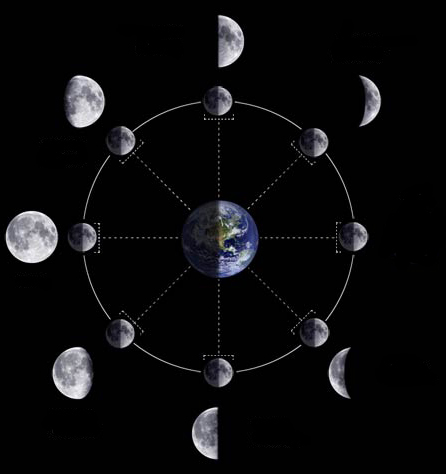
\includegraphics[width=0.95\textwidth]{phases.jpg}
\EC
\column{0.3\textwidth}
\large
You can figure all of this out by drawing pictures.

\bigskip
\bigskip
\bigskip

{\bf \color{Red}Do this} on warmup problems, tutorials, exams...

\bigskip
\bigskip
\bigskip

\end{columns}
}

\frame{

\Huge \BC Complete {\it Lecture Tutorials} pp. 81-88.\EC

}

\frame{

\Huge

When the waxing half moon is just rising over the horizon, it is closest to:

\bigskip
\bigskip
\bigskip

\color{A}A: 6AM \\
\color{B}B: Noon \\
\color{C}C: 6PM \\
\color{D}D: Midnight
}

\frame{

\Huge

As seen from Canada, which part of a waning crescent moon will be lit?

\bigskip
\bigskip
\bigskip

\color{A}A: The right part \\
\color{B}B: The left part \\
}

\frame{\frametitle{\textbf{Oddities in the sky}}

\Large

So far we've talked about the Sun, the Moon, and the stars. What about...

\pause

\BI
\item{planets}
\pause
\item{comets}
\pause
\item{eclipses}
\pause
\item{meteors}
\pause
\item{...}
\EI
}

\frame{\frametitle{\textbf{The planets: what has gone wrong?}}

\Large
\BC
Demo on {\it Stellarium}
\EC

\pause
\bigskip


Sometimes some planets appear to go backwards (``retrograde motion''). 

\bigskip
\bigskip

\large

This tells us that celestial sphere model can't be literally true. Why does it work for everything else?

\BI
\item{The celestial sphere model works if things appear to only rotate around the Earth.}
\item{The stars are so far away that only the Earth's rotation matters}
\item{The Earth orbits the Sun, so we just pretend that the Sun is on a different sphere turning a bit slower, taking into account both our revolution around it and our rotation}
\item{The Moon orbits the Earth, so we again put the Moon on a different sphere, turning slower}
\item{... but how can we get a sphere to go forwards and backwards?}
\item{\bf The celestial sphere model gets the motion of the planets badly wrong}
\EI
}

\frame{\frametitle{\textbf{Oh, you sweet summer child...}}
\Large
\BC
Why are the changes in the seasons in {\it Game of Thrones} so terrifying?
\EC

\pause 
\bigskip
\bigskip
\bigskip

... they're unpredictable!

\bigskip

We've long used the immutability of the sky as a symbol for constancy. The cycles of the Sun, Moon, and stars don't ever change, but some things do!

\bigskip

These unexpected things in the sky once terrified people; now we know why they happen.

}

\frame{\frametitle{\textbf{Eclipses}}
\large
You know that during a new moon, the Moon lies roughly between the Earth and the Sun.

\bigskip

However, the Moon's orbit is tilted just a bit, so it usually passes over or under the Sun.

\bigskip

\BC 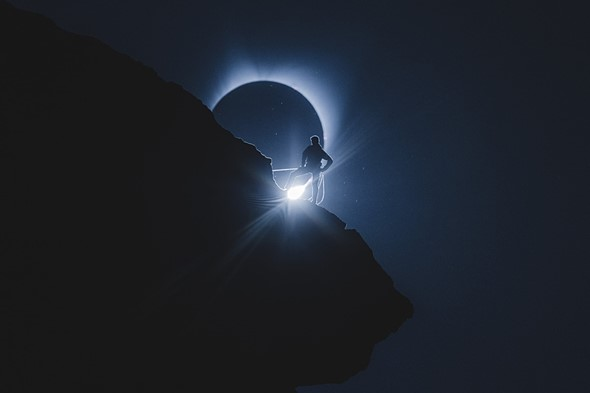
\includegraphics[width=0.6\textwidth]{viralclimber1.jpeg}\EC

\bigskip
\BC
If it passes in front, you get a solar eclipse!

This terrified many of the ancients -- ``the Sun got eaten! We're doomed!''
\EC
}


\frame{\frametitle{\textbf{Eclipses}}
\Large
You know that during a full moon, the Earth lies roughly between the Moon and the Sun.

\bigskip
\bigskip
\bigskip

Same deal: usually the Earth's shadow misses the Moon. Sometimes it doesn't!

\bigskip

\BC 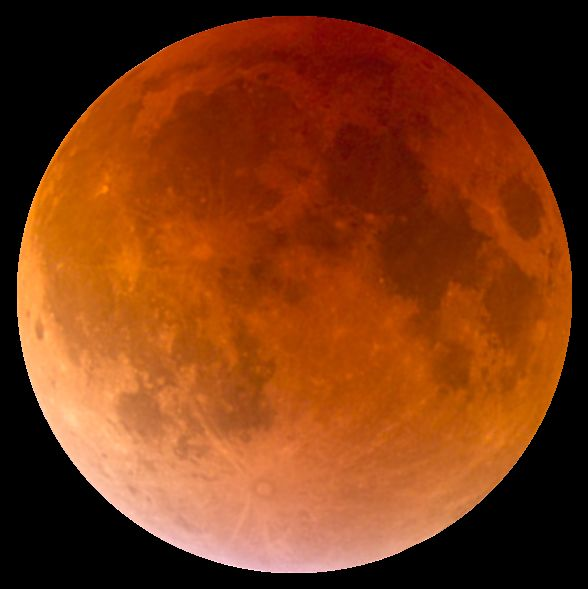
\includegraphics[width=0.27\textwidth]{lunar-eclipse.jpg}\EC

\bigskip

\large

Here some light is refracted by the atmosphere. The blue component is scattered away by the atmosphere; the red component bends and hits the Moon.

}

\frame{\frametitle{\textbf{Meteors}}

\large

Orbits of things in the Solar System are not always close to circular.

\bigskip

There are lots of small things in the Solar System, many of which have elongated orbits that sometimes cross ours.

\bigskip

Meteors:

\large

\begin{columns}
\column{0.6\textwidth}

\BI
\item{Little rocky or metallic bits of matter that orbit the Sun}
\item{Sometimes they get to Earth and glow as atmospheric drag heats them}
\item{Sometimes they hit the surface, and we get chunks of space-slag}
\item{Historical cultures sometimes used them as easy access to metal}
\EI
\column{0.4\textwidth}
\BC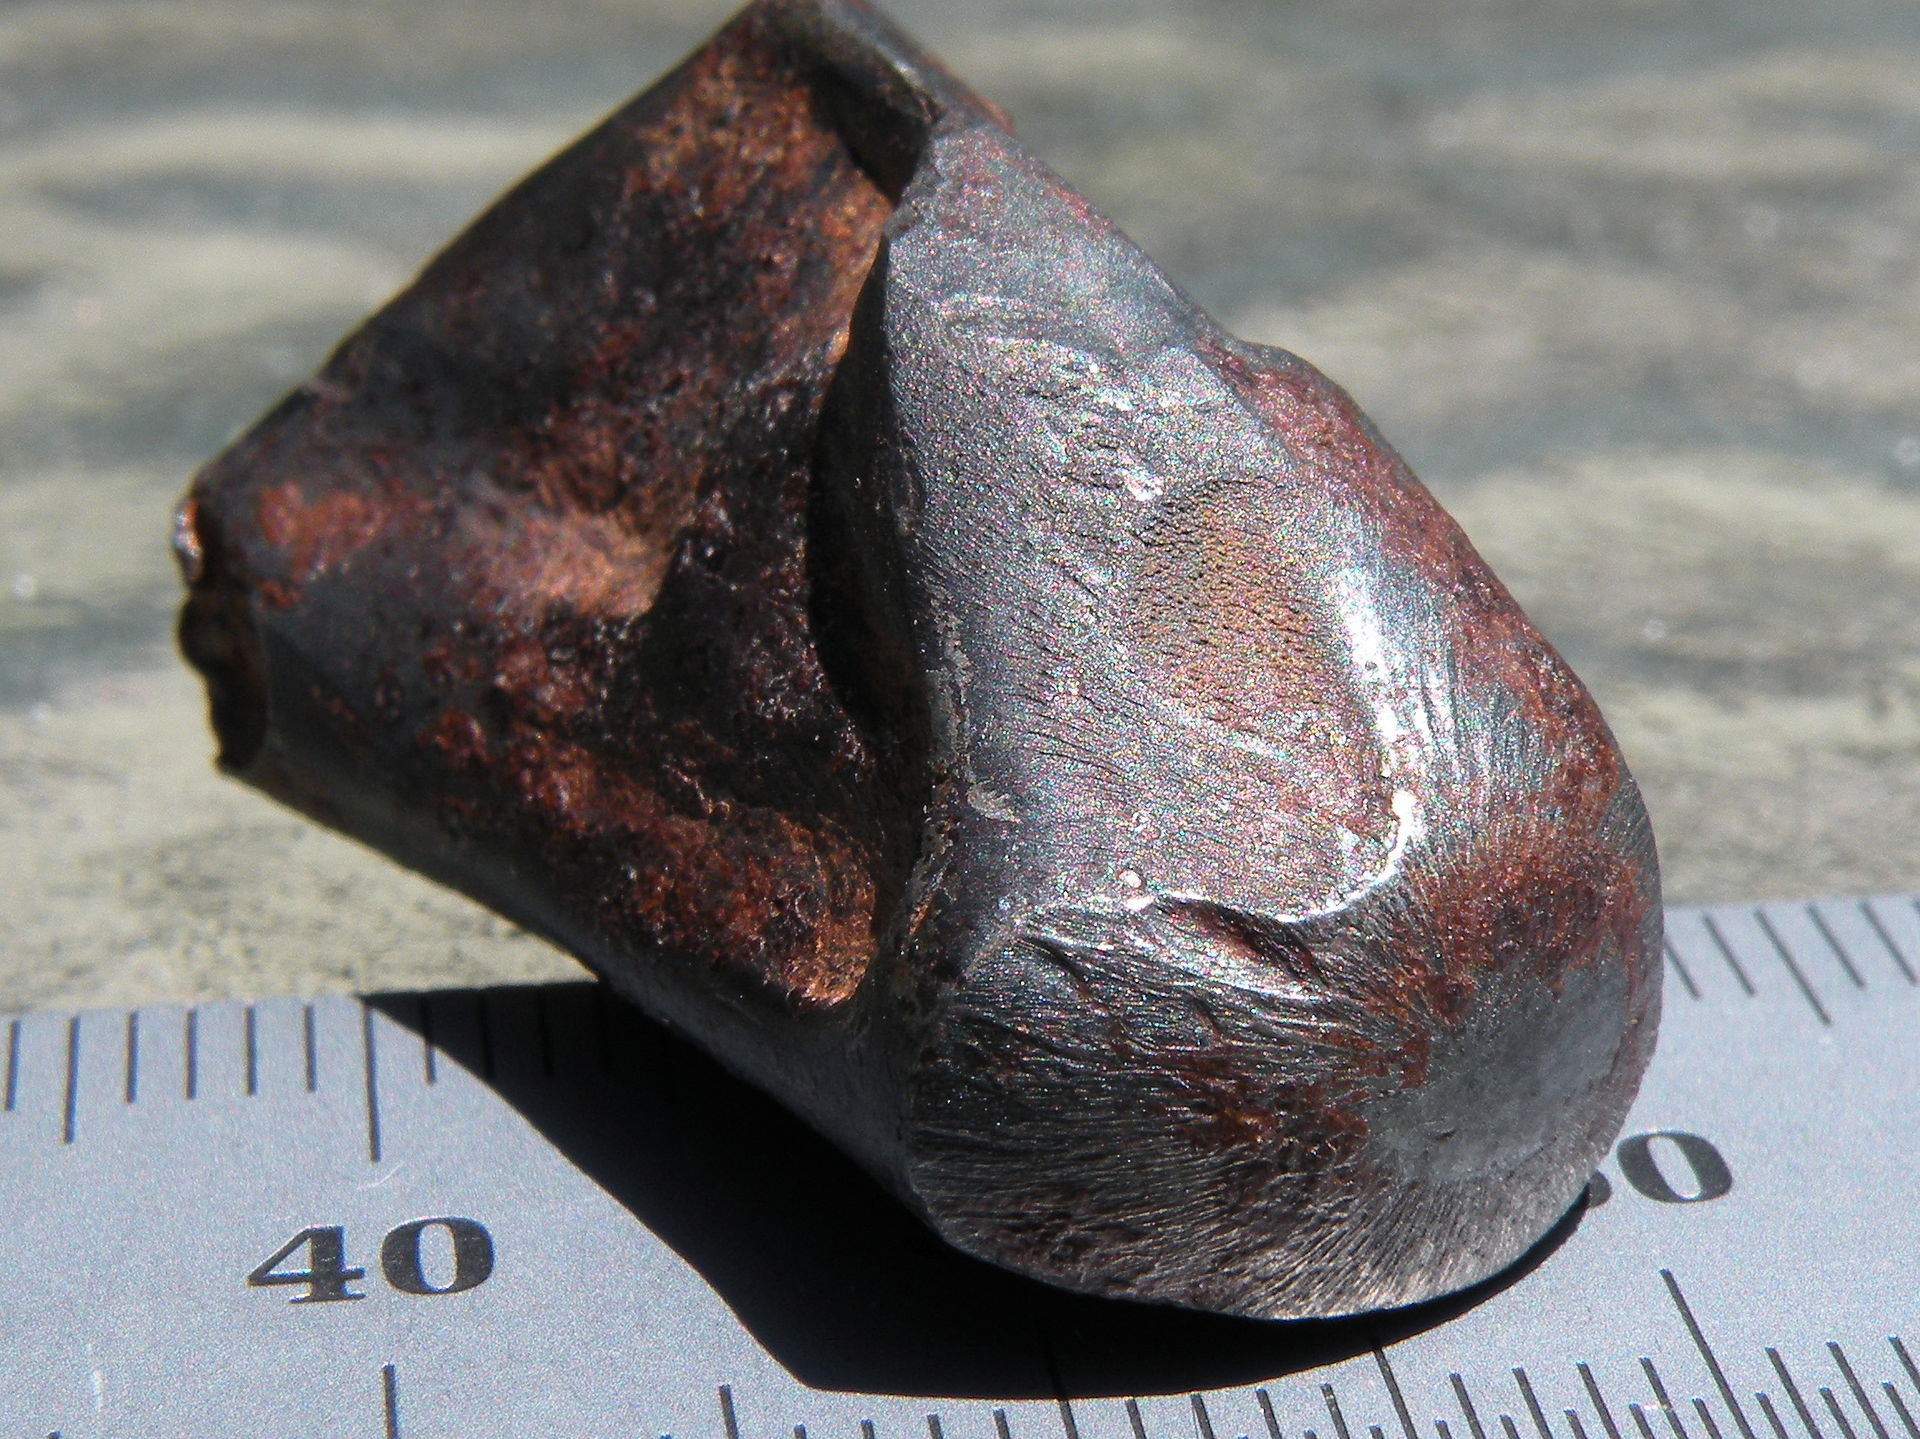
\includegraphics[width=\textwidth]{meteorite.jpg}\EC
\end{columns}
}

\frame{\frametitle{\textbf{Comets}}

\Large

Comets are ``dirty snowballs'' whose orbits are {\it highly} elongated.

\large

\begin{columns}
\column{0.6\textwidth}

\BI
\item{Mostly made of ice}
\item{When they get close to the Sun, the heat melts bits off of them}
\item{This stream of stuff reflects sunlight and makes the comet's ``tail''}
\item{Historical cultures were often terrified of them, but they're just space-snowballs}
\EI
\column{0.4\textwidth}
\BC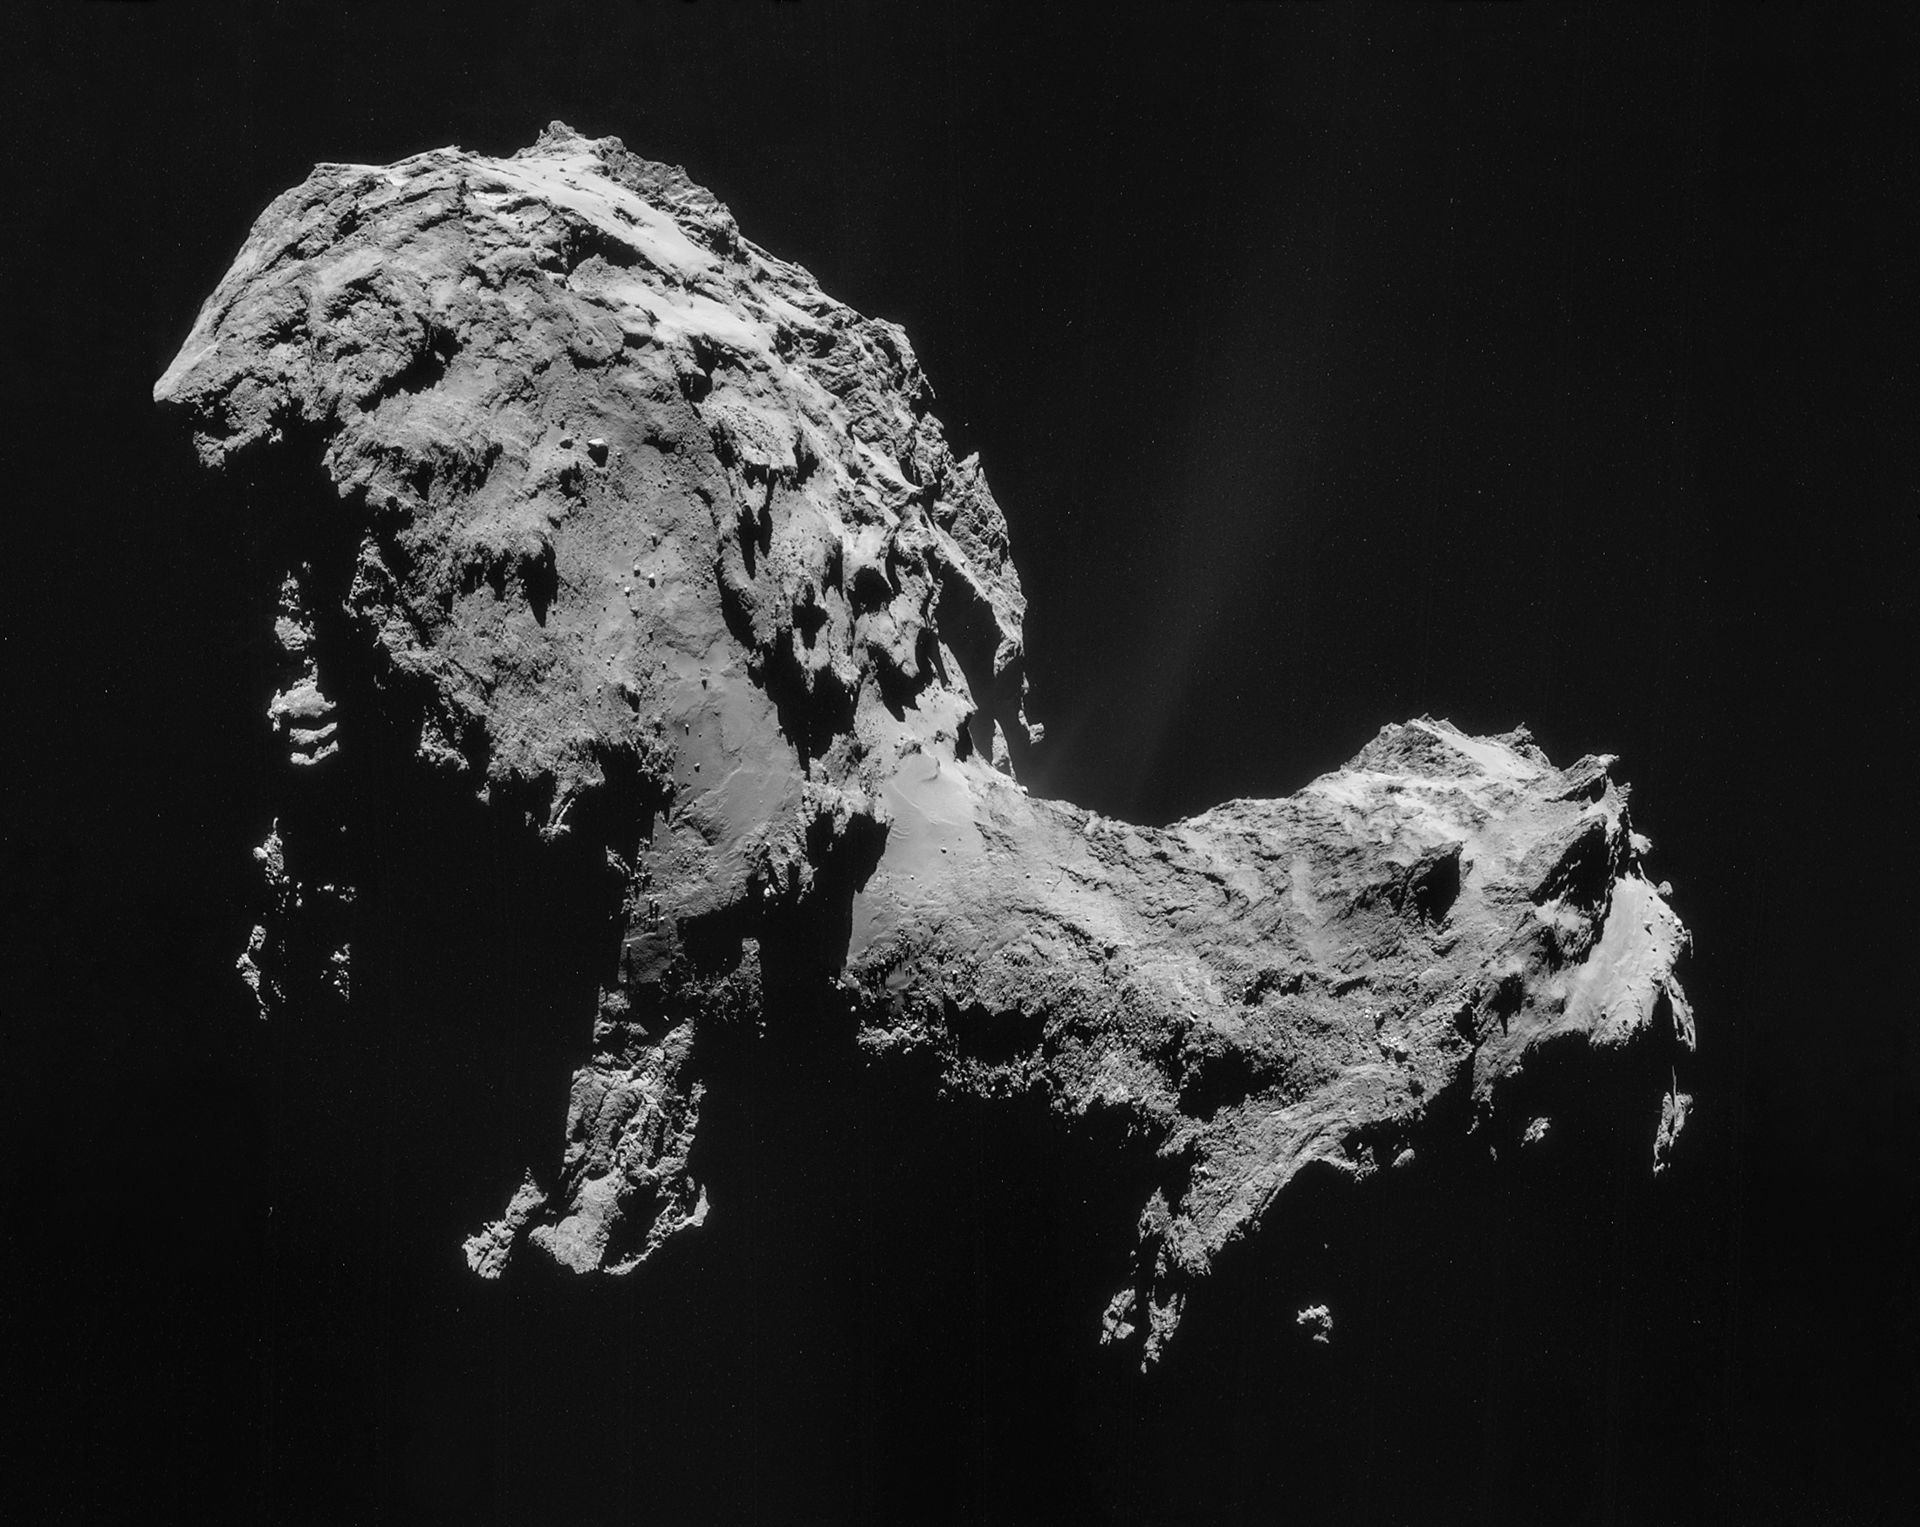
\includegraphics[width=\textwidth]{comet-rosetta.jpg}\EC
\end{columns}
}

\frame{\frametitle{\textbf{The exam}}

\Huge
\BI
\item{Around 30 multiple choice questions}
\item Bring:
\BI
\Large
\item A pencil
\item Knowledge of your SUID (or your student ID card)
\item A single side of an 8.5x11 page of handwritten notes
\item Your blow-up Earth
\EI
\EI
}

\frame{\frametitle{\textbf{The exam: what to study}}
\Large

The exam covers, in descending order of emphasis:


\BI
\item{The material in the {\it Lecture Tutorials}}
\item{The material in the labs}
\item{The material we talked about in class that was {\it not} in the Lecture Tutorials, including demos, videos, etc.}
\item{The material in the textbook}
\item Most importantly, the stuff in Chapter 1 giving a sense of scale about the Solar System and Universe.
\EI

}

\frame{

\BC\Huge Any questions?\EC

}

\end{document}

